In this paper we explore the general utility of certain irregular spherical
topologies beyond offering greater control over network size. We develop and
test new diagnostics to measure and visualize topology-induced errors in SOM.
More specifically we 

\begin{enumerate}
\item Compare the internal heterogeneity of observations captured by a given neuron to that neuron's first-order neighborhood size.
\item For different topologies, compare the internal heterogeneity of each neuron against a composite measure of topological regularity.
\item Develop a SOM-based visualization of the internal heterogeneity.
%\item Develop a reverse quantization error visualization by mapping neurons back onto the input data.
\end{enumerate}

These diagnostics help facilitate the evaluation of both traditional and
spherical SOMs. To satisfy the objective of this research, we apply these
diagnostics to a series of comparable SOMs. Each SOM is trained using the
same synthetic data and training parameters, but utilize different network
topologies. By formally testing for difference of means and variance in the
results of the diagnostics, the following questions are addressed:

\begin{enumerate}
\item Does the internal heterogeneity of a neuron decrease as its first-order neighborhood size, or degree, increases?
\item Is the average internal heterogeneity of a SOM higher when a more irregular topology is used?
\item Which insights, if any, can be gained from a SOM-based visualization of internal heterogeneity?
\end{enumerate}

In traditional SOMs, outlying observations are pushed to the edge of the map
where they encounter fewer competing signals.
%A prime example of this is the ``Utah-Hawaii'' case shown in Figure \ref{f:edge}.  Relying only on the SOM, one would be left to believe that the two states are similar.  The quantiziation error (QError) measures the distance between two vectors in attribute space.  We see that the QError from Utah to the neuron is $1.509$, the QError from Hawaii to the neuron in $1.505$, but the QError from Utah to Hawaii is $3.014$.
Where multiple observations land on the same neuron, it is possible to measure
the average pairwise QErrors between those observations.  This gives us a
notion of internal heterogeneity, \(H\), for each neuron.  We define the
internal heterogeneity of neuron \(i\) as,
 \begin{equation}
   {H_i} = \frac{2}{{n_i}^2-{n_i}}\sum_{j=1}^{n_i}\sum_{k=j+1}^{n_i} ||{x_{ij}}-{x_{ik}}||
 \label{eqno1}
 \end{equation}
where, \(n_i\) is the number of observations mapped to \(i\), and \(x_i\) are
the input vectors mapped to \(i\).  For any neuron that captures more then one
observation, this measure tells how dissimilar those observations are.  This
messure is used in our three diagnostics.

We train SOMs using four different topologies:
\emph{rectangular, hexagonal, geodesic sphere} and \emph{spherical}.  The spherical
topology is based on a method, developed by \cite{Rakhmanov94}, for
distributing an arbitrary number of points on to the surface of a sphere.
Delaunay triangulation is then applied to these points, producing a
topological structure.  To yield meaningful results these SOMs must be trained
with comparable parameters.  The literature provides many rules of thumb for
training a SOM: each SOM is trained in two stages, the first of which uses a larger
initial learning rate and neighborhood search radius with a small number of
training steps; the second stage uses a lower initial learning rate and
neighborhood search radius, but extends the length of training.

As shown in Figure \ref{fig:nSize}, topologies differ in terms of achievable
network size.  For comparability, the network size of each SOM needs to be as
close as possible.  The achievable network size for the geodesic SOM is the
most limiting of the topologies we test. We chose the eighth frequency
geodesic sphere, which has 642 nodes, which is relatively close to the
644-node hexagonal and rectangular topologies achieved when the dimensions are
set to \(28x23\). Finally, the spherical topology was set to 642 nodes.

\begin{figure}[htb]
  \begin{center}
\caption{SOM Size and spherical topologies.}
\label{fig:nSize}
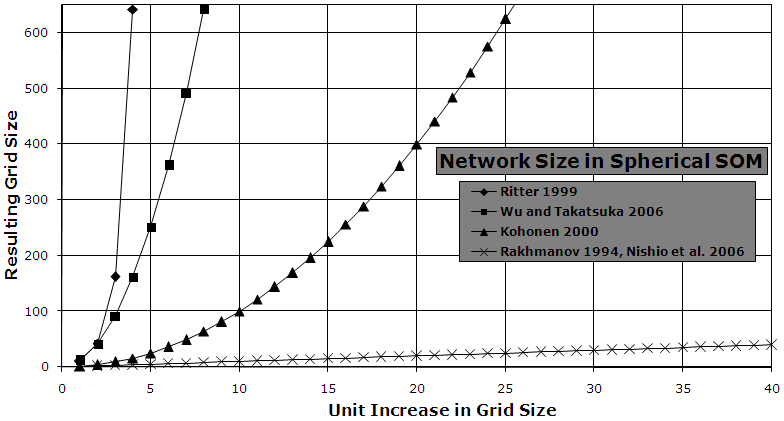
\includegraphics[width=0.70\linewidth]{networkSize.png}
\end{center}
\end{figure}




